\documentclass{beamer}
\usetheme{Antibes}
\AtBeginSection[]{
  \begin{frame}
  \vfill
  \centering
  \begin{beamercolorbox}[sep=8pt,center,shadow=true,rounded=true]{title}
    \usebeamerfont{title}\insertsectionhead\par%
  \end{beamercolorbox}
  \vfill
  \end{frame}
}
\usepackage[utf8]{inputenc}

\newcommand{\bi}{\begin{itemize}}
\newcommand{\ei}{\end{itemize}}
\newcommand{\bis}{\begin{itemize}[<+->]}
\newcommand{\eis}{\end{itemize}}

\newcommand{\indep}{\ensuremath{\perp\mkern -10mu \perp}}
\newcommand{\notindep}{\ensuremath{\perp\mkern -10mu \perp \mkern -17mu \not \mkern 17mu}} % 

\iffalse

Script:

Basics
    - Refresh: random variable, ensemble, marginal probability, conditional, product rule, sum rule, Bayes theorem, independence. [10]
    - Ex. Bayes theorem: clinical tests: sensitivity, specificity, prevalence, posterior probability [10]
   
Forward vs Inverse probabilities
    - Ex. urns: forward calculation, inverse calculation [10]

Learning as Inference (Bayes 1)
    - Terminology
	Bayes theorem: posterior over parameters given data
        - likelihood: a function of parameters, 
        - prior: 
        - evidence: 
    - Bayesian prediction
2.7., 2.8., 2.10, 2.11  [5]

[30-35]

    - Ex. particles [10]
    - Ex. bent coin [10]
    - Ex bent coin model comparison [10]
	
[30-35]

Ex. Legal evicence [10]
Ex. Three doors, normal rules [10]




    - dual view (minimizing error is equivalent to maximizing likelihood)
Supervised
	Bayesian Linear Regression

Unsupervised
	Gaussian Mixture Model

[30]

Chapter 28

sequence [10]



\fi

\title{Machine Learning}
\author{Anders Jonsson, \textbf{Vicenç Gómez}}

\institute{Master in Intelligent Interactive Systems\\
2021-22}

\date{Lecture 9\\Bayesian Machine Learning}

\begin{document}

\maketitle

\section{Introduction}

\begin{frame}
  \frametitle{Introduction}
  \begin{itemize}
    \item Two lectures on Bayesian Machine Learning
    \begin{enumerate}
        \item Learning as Inference (Today)
        \item Inference in Probabilistic Graphical Models (next week)
    \end{enumerate}
    \item Material for Today: \\
    D. Mackay's book: \emph{Information Theory, Inference, and Learning Algorithms}\\
    Chapters 2,3, and 28.
  \end{itemize}
\end{frame}

\begin{frame}
  \frametitle{Introduction}
  \begin{itemize}
    \item Goals of this lecture:
    \begin{itemize}
        \item Refresh basic probability
        \item Inverse probabilities vs forward probabilities
        \item Learning a model as inference
        \item Model comparison as inference (Occam's razor)
        \item Relate this with what you learned so far
    \end{itemize}
  \end{itemize}
\end{frame}


\section{Inverse Probabilities}


\begin{frame}
	\frametitle{Recap on probability theory}
    \textbf{Definitions:}
    \bis
    \item $X$ is a \textbf{random variable}, takes values $x\in\mathcal{A}_X=
        \{a_1,a_2,\hdots,a_i,\hdots,a_I\}$ with probabilities 
        $\mathcal{P}_X=\{p_1,p_2,\hdots,p_i,\hdots,p_I\}$
        \bi
        \item $p(x=a_i)=p_i, p_i \geq 0$
        \item $\sum_{a_i\in\mathcal{A}_X}P(x=a_i)=1$
        \ei
    \item Probability of a \textbf{subset}:
    if $T$ is a subset of $\mathcal{A}_X$ then:
    $P(T) = P(x\in T) = \sum_{a_i\in T}P(x=a_i)$
    \item if $XY$ is an ordered pair of variables where 
%    $x\in \mathcal{A}_X=\{a_1,a_2,\hdots,a_i,\hdots,a_I\}$
%    and $\mathcal{A}_Y=\{b_1,b_2,\hdots,b_j,\hdots,b_J\}$,
    then $P(x,y)$ is the \textbf{joint probability} of $x$ and $y$
    \item \textbf{Marginal} probability:
    $P(x=a_i) = \sum_{y\in\mathcal{A}_y} P(x=a_i,y)$
    \item \textbf{Conditional} probability:
    $$P(x=a_i|y=b_j) = \frac{P(x=a_i,y=b_j)}{P(y=b_j)}, \text{if $P(y=b_j)\neq0$}$$
    \eis
\end{frame}


\begin{frame}
	\frametitle{Recap on probability theory}
    \textbf{Example:}\\
	\begin{columns}
  \column{0.3\textwidth}
   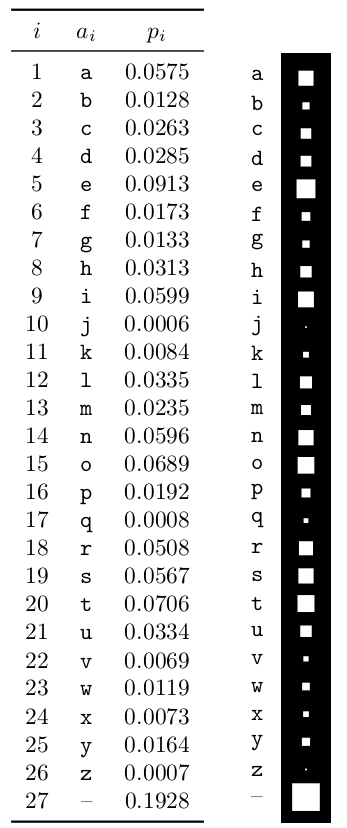
\includegraphics[width=.8\textwidth]{e1}
  \column{0.5\textwidth}
   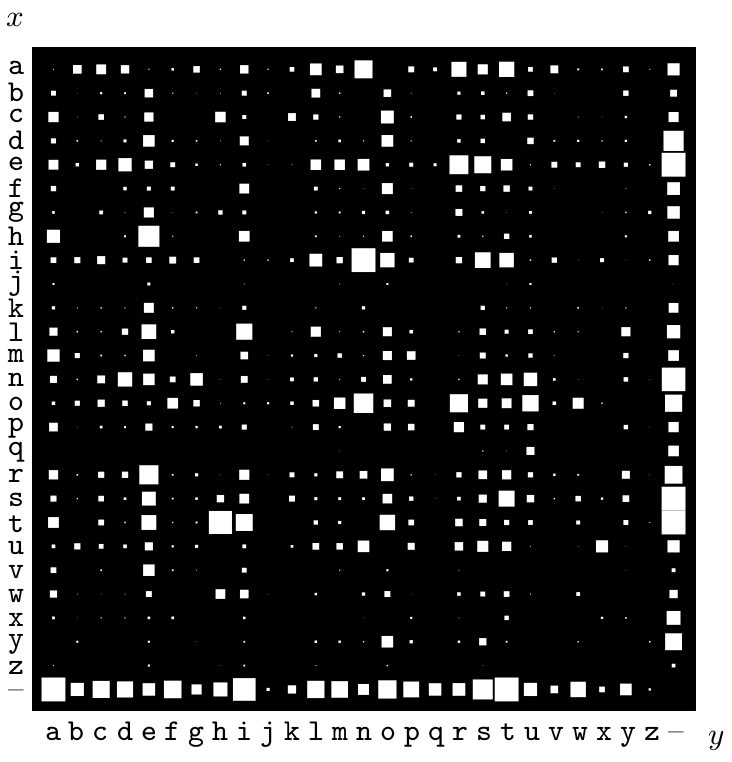
\includegraphics[width=\textwidth]{e2}
  \end{columns}
\end{frame}

\begin{frame}
	\frametitle{Recap on probability theory}
    \textbf{Rules of probability:}
    \bis
    \item Product rule
    $P(x,y)=P(x|y)P(y)=P(y|x)P(x)$
    \item Sum rule
    $P(x)=\sum_y P(x,y) = \sum_y P(x|y)P(y)$
    \item Bayes theorem
    $$P(y|x)=\frac{p(x|y)P(y)}{P(x)}
        =\frac{p(x|y)P(y)}{\sum_{y'}p(x|y')P(y')}$$
    \item Marginal independence: $X$ and $Y$ are independent $X\indep Y|\emptyset$ if and only if
    $$P(x,y)=P(x)P(y)$$
    \item Conditional independence: $X$ and $Y$ are independent given $Z$ 
    $X\indep Y|Z$ if and only if
    $$P(x,y|z)=P(x|z)P(y|z)$$
    \eis
\end{frame}

\begin{frame}
	\frametitle{Recap on probability theory}
    \textbf{Example:}\\
   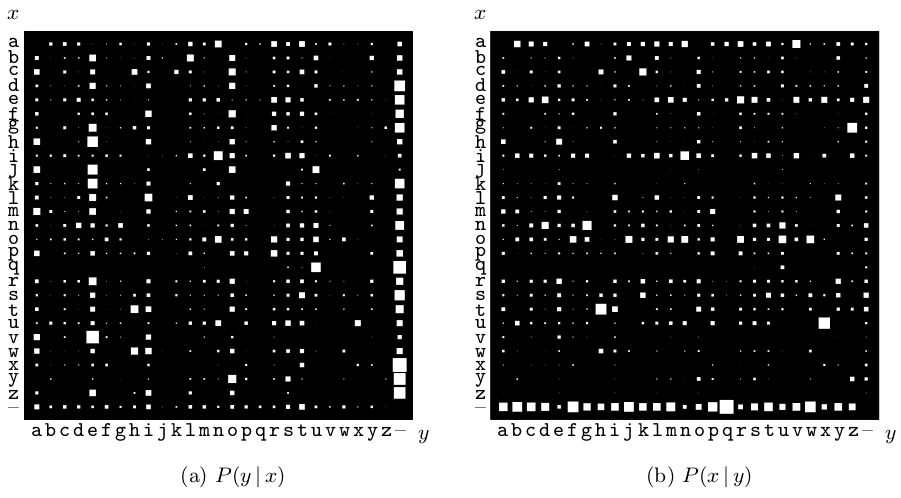
\includegraphics[width=\textwidth]{e3}
 Are $x$ and $y$ independent?
\end{frame}

\begin{frame}
	\frametitle{Recap on probability theory}
    \textbf{Example Bayes (I/II):}\\
   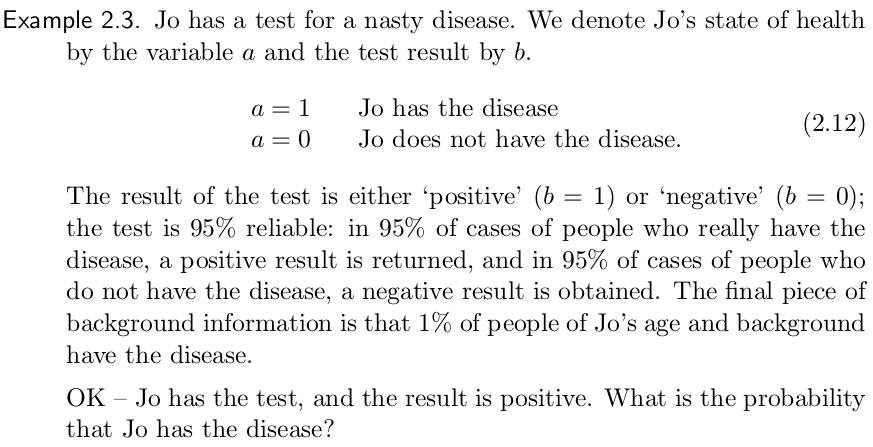
\includegraphics[width=\textwidth]{e4}
\end{frame}

\begin{frame}
	\frametitle{Recap on probability theory}
    \textbf{Example Vaccinations:}\\
  	A negationist tells you that $60\%$ of the people in the hospital with COVID are vaccinated and $40\%$ are not.
	Therefore you should not vaccinate.
	What is wrong with his argumentation?
\visible<2->{
	\begin{enumerate}
	\item $P(v=1|h=1)$ is just one of the three pieces of information.
	We also need to consider the probability of vaccinated and the probability of being in the hospital.
	$$p(h=1|v=1) = \frac{p(v=1|h=1)p(h=1)}{p(v=1)} $$
	\end{enumerate}
}
\end{frame}

\begin{frame}
	\frametitle{Recap on probability theory}
    \textbf{Example Vaccinations:}\\
  	A negationist tells you that $60\%$ of the people in the hospital with COVID are vaccinated and $40\%$ are not.
	Therefore you should not vaccinate.
	What is wrong with his argumentation?
	\begin{enumerate}
	\item $P(v=1|h=1)$ is just one of the three pieces of information.
	We also need to consider the probability of vaccinated and the probability of being in the hospital.
	$$p(h=1|v=1) = \frac{0.6\cdot 0.0001}{0.8}= 7.5\cdot 10^{-5}$$

% 0.8 = p(v=1|h=0)p(h=0) + p(v=1|h=1)p(h=1) )  .8*0.9999 + .6*.0001
	\end{enumerate}
\end{frame}
\begin{frame}
	\frametitle{Recap on probability theory}
    \textbf{Example Vaccinations:}\\
  	A negationist tells you that $60\%$ of the people in the hospital with COVID are vaccinated and $40\%$ are not.
	Therefore you should not vaccinate.
	What is wrong with his argumentation?
	\begin{enumerate}
	\item $P(v=1|h=1)$ is just one of the three pieces of information.
	We also need to consider the probability of vaccinated and the probability of being in the hospital.
	$$p(h=1|v=0) = \frac{0.4\cdot 0.0001}{0.2}= 2\cdot 10^{-4}$$
	\end{enumerate}
\end{frame}

\iffalse
\begin{frame}
	\frametitle{Recap on probability theory}
    \textbf{Example Bayes (II/II):}\\
  	(Hamburgers). Doctors find that people with $KJ$ disease almost invariable ate hamburgers, thus $p(H|KJ)=0.9$.
	The probability that an individual having $KJ$ disease is currently rather low, about one in $100,000$.
	\begin{enumerate}
\item If the fraction of people eating hamburger was rather small, $p(H)=10^{-3}$, what is the probability that a regular hamburger eater will have KJ disease?
	\end{enumerate}
\end{frame}


\begin{frame}
	\frametitle{Recap on probability theory}
\end{frame}


\begin{frame}
	\frametitle{Recap on probability theory}
    \textbf{Example Bayes (II/II):}\\
  	(Hamburgers). Doctors find that people with $KJ$ disease almost invariable ate hamburgers, thus $p(H|KJ)=0.9$.
	The probability that an individual having $KJ$ disease is currently rather low, about one in $100,000$.
	\begin{enumerate}
\item If the fraction of people eating hamburger was rather small, $p(H)=10^{-3}$, what is the probability that a regular hamburger eater will have KJ disease?
	\end{enumerate}
\end{frame}

\fi

\section{Inverse Probabilities}

\begin{frame}
	\frametitle{Forward and inverse probabilities}
	\begin{itemize}
	\item Forward probabilities: given a \emph{generative model}, compute distribution of \emph{data produced} by the model  
	\end{itemize}
Example:\\
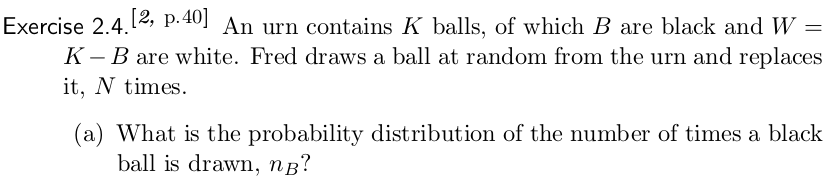
\includegraphics[width=\textwidth]{e5}

\end{frame}


\begin{frame}
	\frametitle{Forward and inverse probabilities}

	\begin{itemize}
	\item Inverse probabilities: given a \emph{generative model}, compute distribution of \emph{hidden variables} in the model, from the observed data  
	\end{itemize}
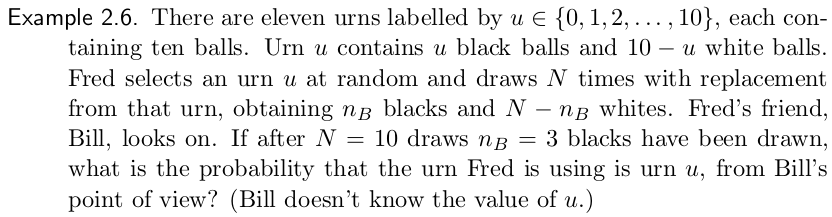
\includegraphics[width=\textwidth]{e6}
\end{frame}



\begin{frame}
	\frametitle{Forward and inverse probabilities}

\end{frame}


\begin{frame}
	\frametitle{Forward and inverse probabilities}
	\begin{columns}
  \column{0.45\textwidth}
   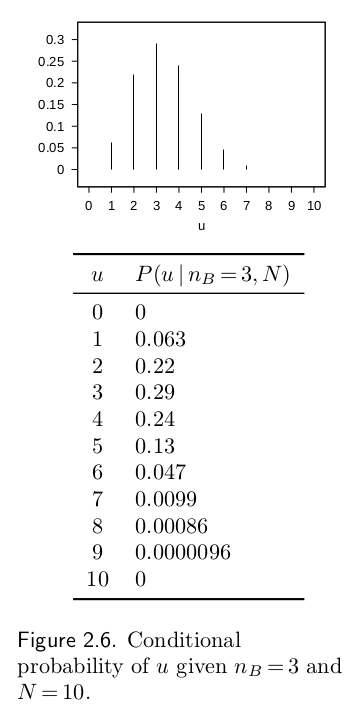
\includegraphics[width=.7\textwidth]{e7}
  \column{0.5\textwidth}
   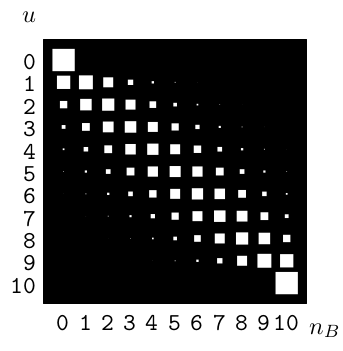
\includegraphics[width=.8\textwidth]{e8}
  \end{columns}
\end{frame}



\begin{frame}
	\frametitle{Forward and inverse probabilities}
	Terminology
	\begin{itemize}[<+->]
	\item $P(u)$ \emph{prior over $u$} (encodes prior knowledge about our model)
	\item $P(n_B|u,N)$ \emph{likelihood of $u$} (NOT likelihood of $n_B$!!)
	\item $P(u|n_B,N)$ \emph{posterior probability} of $u$ given $n_B$
	\item $P(n_B|N)$ \emph{evidence or marginal likelihood} of $n_B$
	\end{itemize}
\end{frame}


\begin{frame}
	\frametitle{Forward and inverse probabilities}
	Terminology
	\begin{itemize}
	\item $P(u)$ \emph{prior over $u$} (encodes prior knowledge about our model)
	\item $P(n_B|u,N)$ \emph{likelihood of $u$} (NOT likelihood of $n_B$!!)
	\item $P(u|n_B,N)$ \emph{posterior probability} of $u$ given $n_B$
	\item $P(n_B|N)$ \emph{evidence or marginal likelihood} of $n_B$
	\end{itemize}
\begin{block}{Bayes I}
$$ P(\boldsymbol{\theta}| \mathcal{D}, \mathcal{H}) = \frac{P(\mathcal{D}|\boldsymbol{\theta}, \mathcal{H})P(\boldsymbol{\theta}|\mathcal{H})}{P(\mathcal{D}|\mathcal{H})}$$
\end{block}
\end{frame}


\begin{frame}
	\frametitle{Forward and inverse probabilities}
	Inverse probability and prediction
	\begin{itemize}
	\item Involves \emph{marginalizing} over possible values of the hypothesis
	\end{itemize}
   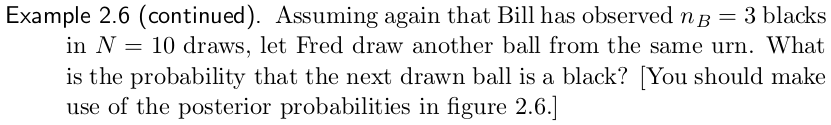
\includegraphics[width=.8\textwidth]{e9}
\end{frame}



\begin{frame}
	\frametitle{Forward and inverse probabilities}
	1st set of exercises for next week.
	From chap. 2 of D. Mackay
	\begin{itemize}
	\item 2.7.
	\item 2.8.
	\item 2.10.
	\item 2.11.
	\end{itemize}

\end{frame}

\section{Learning as Inference (Bayes I)}

\begin{frame}
	\frametitle{Learning as inference}
   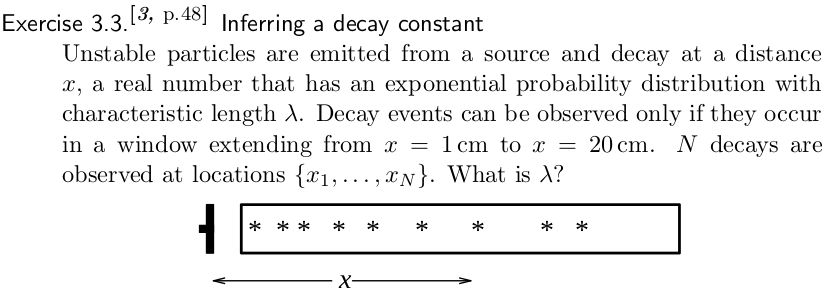
\includegraphics[width=\textwidth]{e10}
\end{frame}


\begin{frame}
	\frametitle{Learning as inference}
\end{frame}


\begin{frame}
	\frametitle{Learning as inference}
   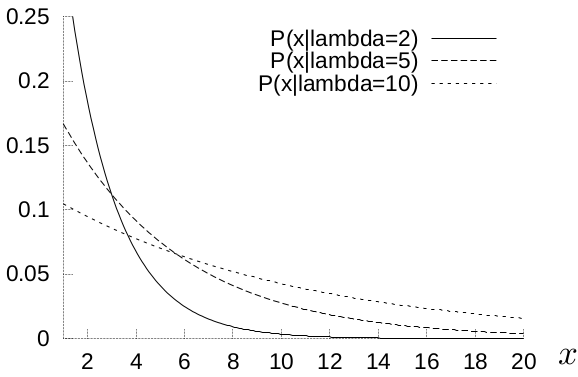
\includegraphics[width=.8\textwidth]{e11}\\
	The probability density $p(x|\lambda)$ (a truncated exponential)
\end{frame}

\begin{frame}
	\frametitle{Learning as inference}
   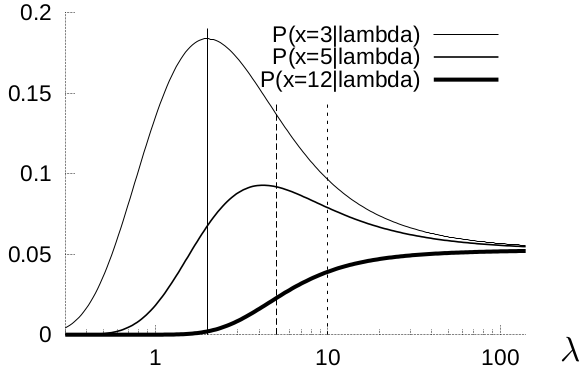
\includegraphics[width=.8\textwidth]{e12}\\
     The likelihood function $p(x|\lambda)$ for one data point
\end{frame}

\begin{frame}
	\frametitle{Learning as inference}
   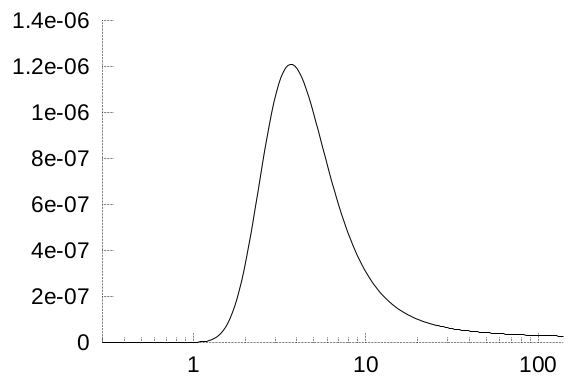
\includegraphics[width=.8\textwidth]{e13}\\
	The likelihood function for $\mathcal{D}=\{1.5,2,3,4,5,12\}$
\end{frame}


\begin{frame}
	\frametitle{Learning as inference}
	\begin{block}{Bayesian Linear Regression}
	\begin{itemize}
	\item Remember linear regression: find $w$ that minimizes
$$L_S(w) =\frac{1}{m} \sum_{i=1}^m (y_i-w^\top x_i)^2 $$
	\end{itemize}
	\end{block}
\end{frame}



\begin{frame}
	\frametitle{Learning as inference}
	\begin{block}{Bayesian Linear Regression}
	\begin{itemize}
	\item Data points generated as noisy targets $y_i \sim w^\top x_i + \eta$
	\item If noise is Gaussian, $\eta \sim \mathcal{N}(0,\sigma^2)$, the model generates $y_i$
	\begin{align*}
	p(y_i|x_i,w) & = \mathcal{N}(w^\top x_i,\sigma^2) \\
			& = \frac{1}{\sqrt{2\pi\sigma^2}}\exp\left(-\frac{1}{2\sigma^2}(y_i-w^\top x_i)^2 \right)
	\end{align*}
	\item For $m$ i.i.d. datapoints, the likelihood becomes
	$$p(\mathcal{D} | w) = \prod_{i=1}^m p(y_i|x_i,w)p(x_i)$$
	\end{itemize}
	\end{block}
\end{frame}


\begin{frame}
	\frametitle{Learning as inference}
	\begin{block}{Bayesian Linear Regression}
	\begin{itemize}[<+->]
	\item Ignoring $1/\sigma^2$ and the input distribution $p(x_i)$, taking $\log$
	$$\log p(\mathcal{D} | w) = -\sum_{i=1}^m (y_i-w^\top x_i)^2$$
	\item \textbf{Minimizing squared error is equivalent to maximizing the likelihood under Gaussian noisy outputs}
	\item What are we missing?
	\end{itemize}
	\end{block}
\end{frame}

\begin{frame}
	\frametitle{Learning as inference}
	\begin{block}{Bayesian Linear Regression}
	\begin{itemize}[<+->]
	\item The priors!
	\item For Gaussian priors $p(w|\lambda)\sim \mathcal{N}(0,1/\lambda^2)$, posterior is
	$$\log p(w| \mathcal{D},\lambda) = -\sum_{i=1}^m (y_i-w^\top x_i)^2 - \lambda w^\top w + \text{const}$$
	\item Remember linear regression with regularization
	$$L_{aug}(w) = \frac{1}{m} \sum_{i=1}^m (y_i-w^\top x_i)^2 + \frac{\lambda}{m} w^\top w$$
	\item \textbf{The prior plays the role of regularization}
	\end{itemize}
	\end{block}
\end{frame}


\section{Model Comparison as Inference (Bayes II)}


\begin{frame}
	\frametitle{Model Comparison}
	How to choose between models / hypothesis?
	\begin{block}{Bayes II}
$$ P( \mathcal{H}| \mathcal{D}) = \frac{P(\mathcal{D}|\mathcal{H})P(\mathcal{H})}  {P(\mathcal{D})}$$
	\end{block}
\end{frame}


\begin{frame}
	\frametitle{Model Comparison}
\begin{block}{Bayes I}
$$ P(\boldsymbol{\theta}| \mathcal{D}, \mathcal{H}) = \frac{P(\mathcal{D}|\boldsymbol{\theta}, \mathcal{H})P(\boldsymbol{\theta}|\mathcal{H})}{{\color{red}P(\mathcal{D}|\mathcal{H})}}$$
\end{block}
	\begin{block}{Bayes II}
$$ P( \mathcal{H}| \mathcal{D}) = \frac{{\color{red}{P(\mathcal{D}|\mathcal{H})}}P(\mathcal{H})}  {P(\mathcal{D})}$$
	\end{block}
	Note that $P(\mathcal{D}|\mathcal{H})$ corresponds to the evidence of Bayes I (a.k.a. \emph{marginal likelihood})
\end{frame}



\begin{frame}
	\frametitle{Model Comparison}
   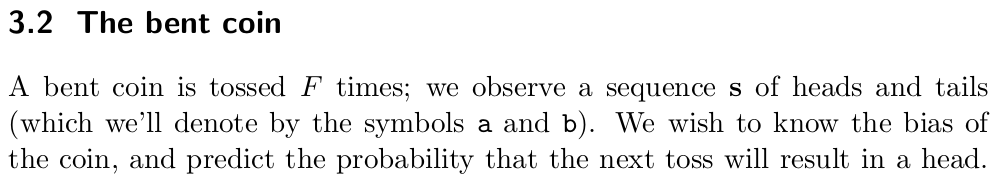
\includegraphics[width=.8\textwidth]{e14}\\
\begin{itemize}
	\item Hypothesis $\mathcal{H}_1$ assumes that there is an unknown bias (parameter) we want to infer
\end{itemize}
\end{frame}


\begin{frame}
	\frametitle{Model Comparison}
\end{frame}

\begin{frame}
	\frametitle{Model Comparison}
\begin{itemize}
\item Posterior is
	$$p(p_a | \mathbf{s}, \mathcal{H}_1) = \frac{p_a^{F_a} (1-p_a)^{F_b}}{p(\mathbf{s}|F,\mathcal{H}_1)} $$
\item Evidence is
	$$p(\mathbf{s} | \mathcal{H}_1) = \int_0^1 dp_a p_a^{F_a} (1-p_a)^{F_b} =\frac{F_a!F_b!}{(F_a+F_b+1)!} $$
\end{itemize}
\end{frame}


\begin{frame}
	\frametitle{Model Comparison}
\begin{itemize}
\item Predictions
	\begin{align*}
	p(\mathtt{a}|\mathbf{s}, \mathcal{H}_1) &= \int_0^1 dp_a p(\mathtt{a}|p_a,\mathcal{H}_1)p(p_a|\mathbf{s},\mathcal{H}_1)\\
	& = \frac{F_a+1}{F_a+F_b+2}
	\end{align*}
\end{itemize}
\end{frame}


\begin{frame}
	\frametitle{Model Comparison}
   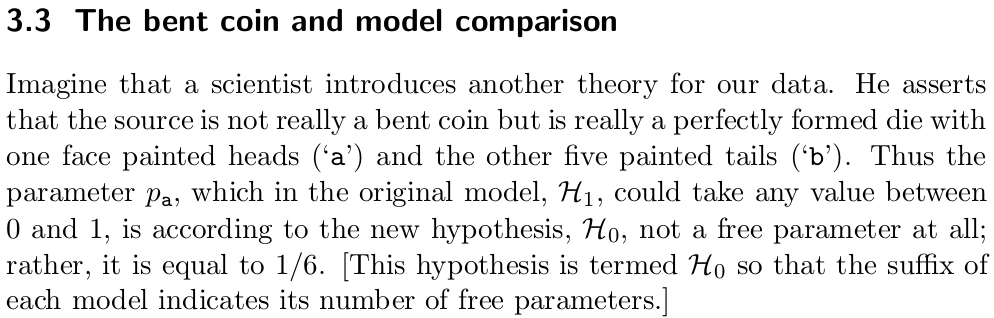
\includegraphics[width=.8\textwidth]{e15}\\
\end{frame}



\begin{frame}
	\frametitle{Model Comparison}
   \begin{itemize}
\item The likelihood under the (simpler) hypothesis $\mathcal{H}_0$ is
	$$p(\mathbf{s}|\mathcal{H}_0) = (1/6)^{F_a} (1-1/6)^{F_b}$$
\item The ratio of posteriors is
	$$\frac{p(\mathcal{H}_1|\mathbf{s})}{p(\mathcal{H}_0|\mathbf{s})} = \frac{F_a!F_b!}{(F_a+F_b+1)!} \frac{1}{(1/6)^{F_a} (1-1/6)^{F_b}}$$
\end{itemize}
\end{frame}


\begin{frame}
	\frametitle{Model Comparison}
   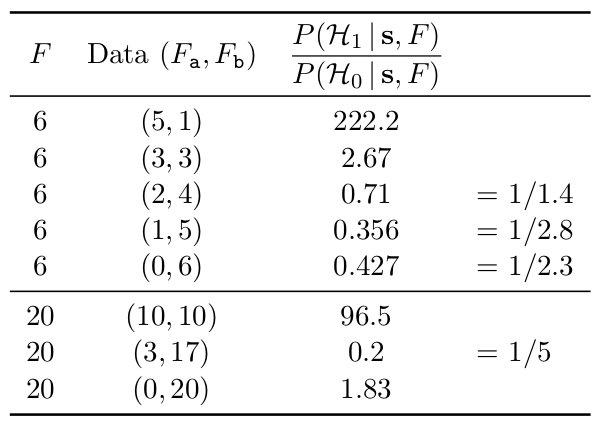
\includegraphics[width=.8\textwidth]{e16}\\
	Some values of $\frac{p(\mathcal{H}_1|\mathbf{s})}{p(\mathcal{H}_0|\mathbf{s})} $ for different data
\end{frame}


\begin{frame}
	\frametitle{Model Comparison}
   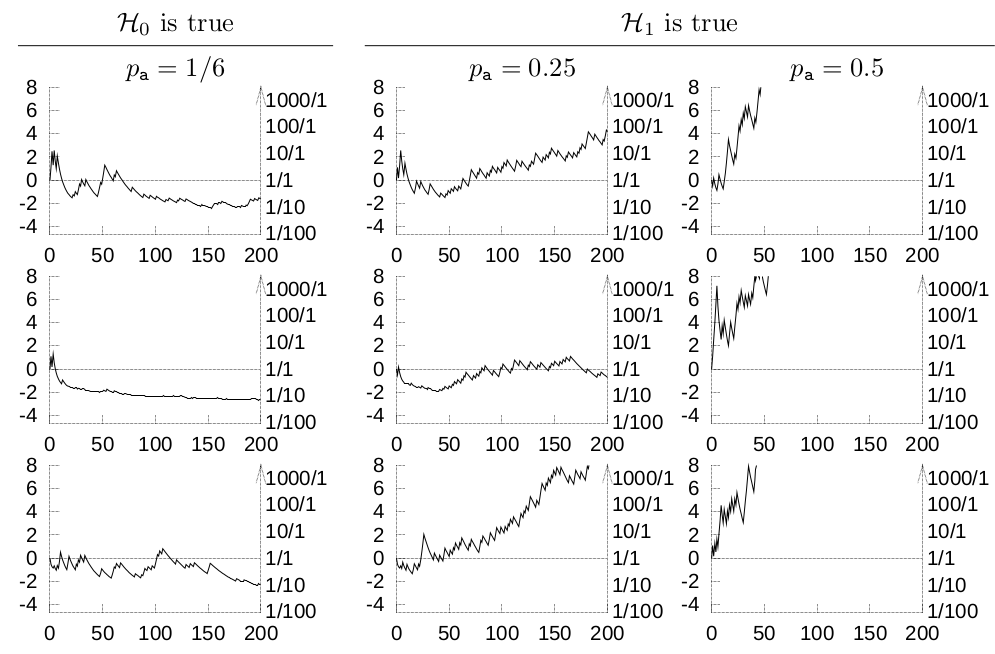
\includegraphics[width=.8\textwidth]{e17}\\
	Behavior as a function of the size of the data
\end{frame}

\begin{frame}
	\frametitle{Model Comparison}
	Example: three doors
   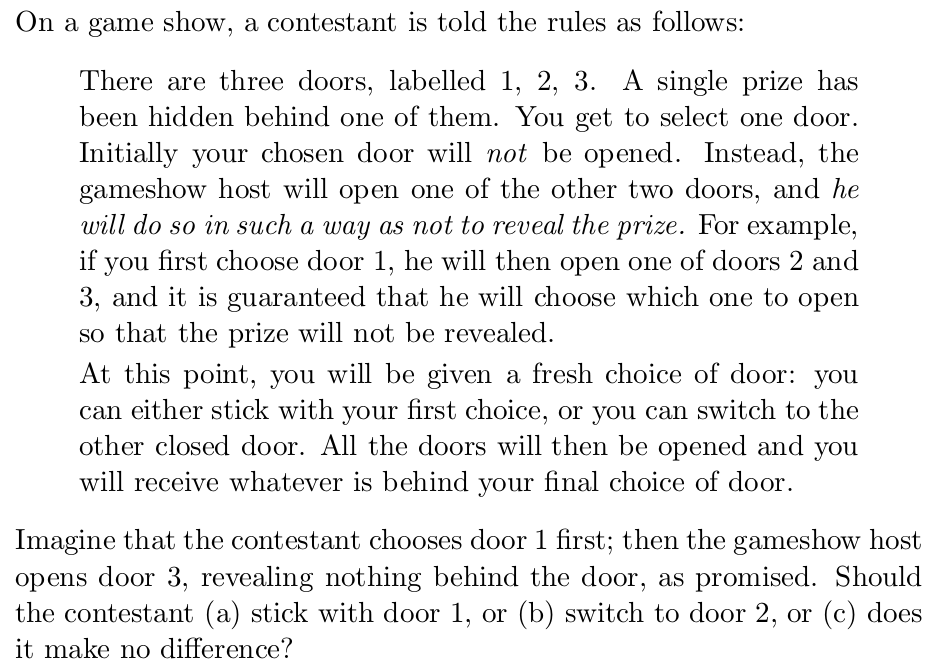
\includegraphics[width=.8\textwidth]{e18}\\
\end{frame}

\begin{frame}
	\frametitle{Model Comparison}
	Example: three doors
\begin{itemize}
\item $\mathcal{H}_i$ : car is at door $i$. $i\in\{1,2,3\}$.
\item Likelihoods
   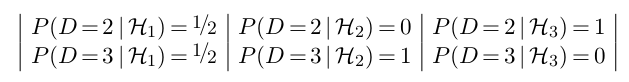
\includegraphics[width=.8\textwidth]{3doors}
\item Posterior\\
   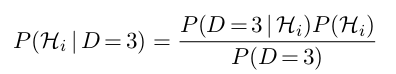
\includegraphics[width=.5\textwidth]{3doors2}
   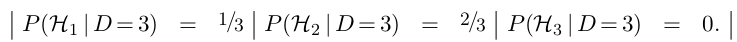
\includegraphics[width=.8\textwidth]{3doors3}
\end{itemize}

\end{frame}

\begin{frame}
	\frametitle{Model Comparison}
\end{frame}

\begin{frame}
	\frametitle{Model Comparison}
	2nd set of exercises for next week.
	From chap. 3 of D. Mackay
	\begin{itemize}
	\item 3.5.
	\item 3.10.
	\item 3.12.
	\item 3.14.
	\end{itemize}

\end{frame}



\begin{frame}
	\frametitle{Occam's razor}
   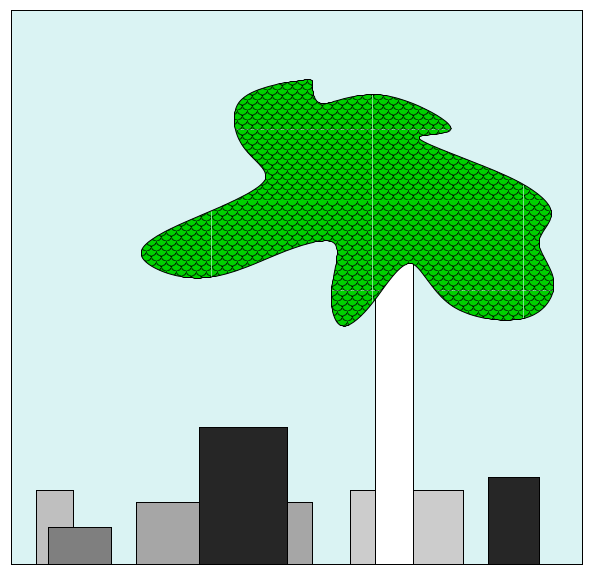
\includegraphics[width=.6\textwidth]{e19}\\
	How many boxes are in the picture?
\end{frame}


\begin{frame}
	\frametitle{Occam's razor}
	\begin{columns}
  \column{0.5\textwidth}
   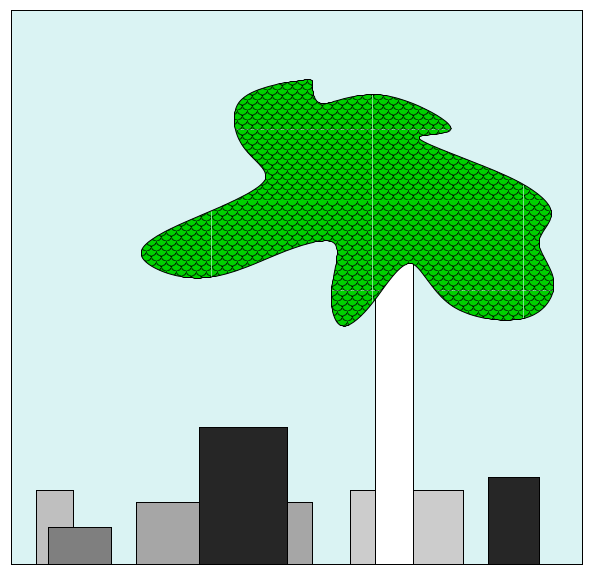
\includegraphics[width=\textwidth]{e19}\\
	How many boxes are in the picture? 
 \column{0.5\textwidth}
   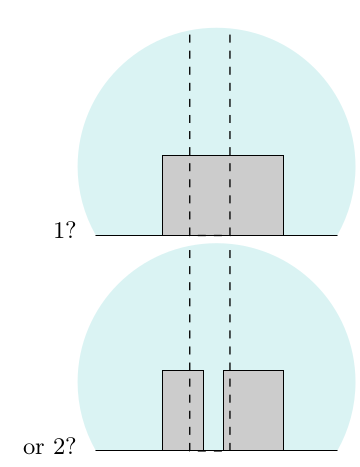
\includegraphics[width=\textwidth]{e20}
  \end{columns}

\end{frame}

\begin{frame}
	\frametitle{Occam's razor}
\begin{itemize}
\item Accept the \emph{simplest} explanation that fits the data
\item Bayesian inference embodies Occam's razor \emph{automatically}
\end{itemize}
   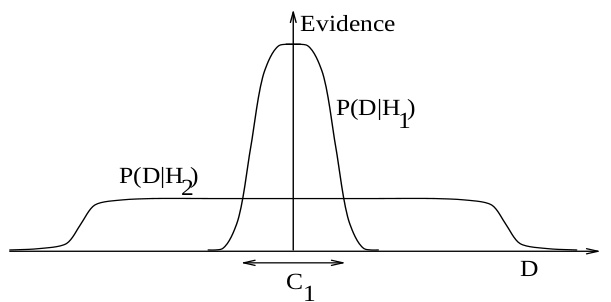
\includegraphics[width=\textwidth]{e21}
\end{frame}

\begin{frame}
	\frametitle{Occam's razor}
   \begin{block}{Example: sequence of numbers}
	\begin{itemize}[<+->]
	\item Given the sequence:
	$$-1,3,7,11$$
	\item What are the next two numbers? What is the generating process? 
	\item Option 1: $(15,19, \hdots)$ \emph{start from $-1$, and add $1$ to the previous number}
	\item Option 2: $(-19.9, 1043.8, \hdots)$ \emph{start from $-1$, use the previous number $x$ to get the new one according to}
	$$ -x^3/11 + 9/11x^2 + 23/11$$ 
	\end{itemize}
\end{block}
\end{frame}

\begin{frame}
	\frametitle{Occam's razor}
         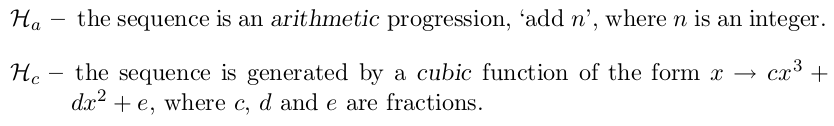
\includegraphics[width=\textwidth]{e22}
	\visible<2->{
	\begin{itemize}
\item Model $\mathcal{H}_a$ has \textbf{two} parameters: first number, and $n$
   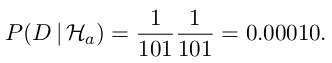
\includegraphics[width=.4\textwidth]{seq1}
\item Model $\mathcal{H}_c$ has \textbf{four} parameters: first number, $c,d$, and $e$
   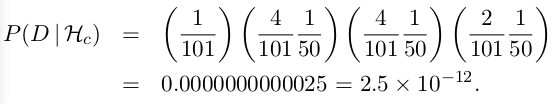
\includegraphics[width=.7\textwidth]{seq2}
\end{itemize}
	}

\end{frame}



\end{document}
